%\documentclass[mathserif]{beamer}
\documentclass[handout]{beamer} 

%\documentclass[handout,mathserif]{beamer} 
\usepackage{pgfpages}  
\usepackage{tikz}
\usepackage{fancybox}
\usetikzlibrary{shapes,chains,scopes,positioning,arrows}
\tikzset{block/.style={draw, rectangle, rounded corners, very thick, text centered}}
  \usetikzlibrary{calc,patterns,
                 decorations.pathmorphing,
                 decorations.markings}
%\include{tikz-3dplot}
\usepackage{3dplot}
%\usepackage[active,tightpage]{preview}  %generates a tightly fitting border around the work
%\PreviewEnvironment{tikzpicture}
%\setlength\PreviewBorder{2mm}

%\pgfpagesuselayout{2 on 1}[a4paper,border shrink=5mm]
%\mode<handout>{\setbeamercolor{background canvas}{bg=black!5}}

%\usetheme{Montpellier}
%\usetheme{Singapore}
\usetheme{Boadilla}

\usepackage{helvet}

%\usepackage{beamerthemeshadow}
\usepackage{amsmath,amssymb,amsthm}
\usetikzlibrary{calc,patterns,decorations.pathmorphing,decorations.markings}
\newcommand{\ra}{\rightarrow}
\newcommand{\ul}{\underline}
\newcommand{\lby}[1]{\stackrel{#1}{\longrightarrow}}

\newcommand{\BA}{\mbox{$\mathbb A$}}    \newcommand{\BB}{\mbox{$\mathbb B$}}
\newcommand{\BC}{\mbox{$\mathbb C$}}    \newcommand{\BD}{\mbox{$\mathbb D$}}
\newcommand{\BE}{\mbox{$\mathbb E$}}    \newcommand{\BF}{\mbox{$\mathbb F$}}
\newcommand{\BG}{\mbox{$\mathbb G$}}    \newcommand{\BH}{\mbox{$\mathbb H$}}
\newcommand{\BI}{\mbox{$\mathbb I$}}    \newcommand{\BJ}{\mbox{$\mathbb J$}}
\newcommand{\BR}{\mbox{$\mathbb R$}}    \newcommand{\BL}{\mbox{$\mathbb L$}}
\newcommand{\BZ}{\mbox{$\mathbb Z$}}
\def\dim{\text{dim}}
\def\Span{\text{Span}}
\def\proj{\text{proj}}

\def\bb{\mathbf b}
\def\bc{\mathbf c}
\def\bd{\mathbf d}
\def\bu{\mathbf u}
\def\bx{\mathbf x}
\def\by{\mathbf y}
\def\bz{\mathbf z}

\def\cB{\mathcal{B}}
\def\cC{\mathcal{C}}
\def\cM{\mathcal{M}}
\def\cS{\mathcal{S}}
\def\cP{\mathcal{P}}
\def\dim{\text{dim }}
\def\Span{\text{Span}}
\def\rank{\text{rank}}
\def\det{\text{det}}

\def\proj{\text{proj}}
\def\b#1{\textbf{#1}}
\def\innp#1#2{\langle #1 \, , #2 \rangle}
\definecolor{olive}{rgb}{0.3, 0.4, .1}
\definecolor{maroon}{RGB}{153,0,0}
\definecolor{dgreen}{RGB}{0,102,0}
\definecolor{NavyBlue}{RGB}{0,0,204}
\definecolor{Magenta}{cmyk}{0,1,0,0}
\definecolor{dblue}{RGB}{0,0,180}

\begin{document} 
\title[D1 - Lecture 19]{ MA-106 Linear Algebra} 
\author{H. Ananthnarayan} 
\institute[]{
\includegraphics[width=0.7in]{iitblogo}\\Department of Mathematics\\Indian Institute of Technology Bombay\\
Powai, Mumbai - 76 }
\date[15th February 2018]{\small{15th February 2018 \\ D1 - Lecture 19}}
\frame{\titlepage}


\begin{frame}
\frametitle{Summary: Diagonalizability}
Let $A$ be $n \times n$. \pause

$\bullet$ $A$ is diagonalizable \pause $\Leftrightarrow$ $\BR^n$ has a basis\pause, say $\cB = \{v_1,\ldots, v_n\}$, of eigenvectors of $A$, \pause
associated to eigenvalues $\lambda_1,\ldots, \lambda_n$. \pause In this case, $P^{-1}AP = \Lambda$, \pause where $P = \begin{pmatrix} v_1 &  \cdots & v_n\end{pmatrix}$ \pause 
and $\Lambda$ is a diagonal matrix with entries $\lambda_1,\ldots, \lambda_n$. \pause\smallskip

$\bullet$ If $A$ is diagonalizable, and $T$ is the linear operator defined by $Tx = Ax$\pause, then $[T]_{\cB}^{\cB} = \Lambda$. \pause
Thus diagonalization of $A$ is the same as \pause finding a basis w.r.t. which the matrix of $T$ \pause (defined by $Tx = Ax$) is diagonal.\pause\smallskip

$\bullet$ Eigenvectors associated to distinct eigenvalues \pause are linearly independent. \pause In particular, if $A$ has $n$ distinct eigenvalues\pause, 
$A$ is diagonalizable. \pause \smallskip

$\bullet$ If $v$ is an eigenvector of $A$ \pause with respect to eigenvalue $\lambda$, \pause then
$v$ is also an eigenvector of $A^k$ \pause w.r.t. eigenvalue $\lambda^k$ for $k \geq 0$. \pause In particular, if $A$ is diagonalizable, \pause and $P^{-1}AP$ is diagonal, the same holds for $P^{-1}A^k P$. \pause These statements hold for all $k \in \BZ$ if $A$ is invertible.
\end{frame}


\begin{frame}{Complex Eigenvalues}

\only<2->{{\bf Ex:} Rotation by $90^o$ in $\BR^2$ is} 
\only<3->{given by $Q=\begin{pmatrix} 0& -1 \\ 1& 0 \end{pmatrix}$.} 

\only<4>{$Qe_1=\_\_$ and $Qe_2 = \_\_$.}\smallskip
\only<5 -10> {It has no eigenvectors} 
\only<6-10>{since rotation by $90^o$ changes the direction.} \smallskip
\only<11-> {It has no \textcolor{red}{real} eigenvectors.}\smallskip

\only<7->{$Q$ has eigenvalues, but they are \textcolor{red}{not  real}.} 
\only<8->{$\det(Q-\lambda I) = $}
\only<9->{$\lambda^2+1$}  
\only<10->{$\Rightarrow$ $\lambda_1 = i$ and $\lambda_2 = -i$, where $i^2=-1$.} 

\only<12->{Let us compute the eigenvectors.} \smallskip

\only<13->{$(Q-iI)x_1= $}
\only<14->{$\begin{pmatrix} -i & -1 \\ 1 & -i\end{pmatrix} x_1 = 0$} 
\only<15->{$\Rightarrow x_1=$}
\only<16->{$\begin{pmatrix}1\\-i \end{pmatrix}$,} \medskip

\only<17->{$(Q+iI)x_2 =$}
\only<18->{$\begin{pmatrix} i & -1 \\ 1 & i\end{pmatrix} x_2=0$}
\only<19->{$\Rightarrow x_2=$}
\only<20->{$\begin{pmatrix}1\\i \end{pmatrix}$.} \medskip

\only<21->{The eigenvalues, though imaginary, are distinct,} 
\only<22->{hence eigenvectors are linearly independent.} \smallskip

\only<23->{If $P=\begin{pmatrix} x_1 & x_2 \end{pmatrix}$} 
\only<24->{$= \begin{pmatrix} 1 & 1\\ -i & i \end{pmatrix}$,} 
\only<25->{ then $P^{-1}QP= \begin{pmatrix} i& 0 \\ 0 & -i\end{pmatrix}$.}
\end{frame}


\begin{frame}{Complex Vectors}\pause

\textcolor{dgreen}{\bf Conclusion:} \pause We need complex numbers $\BC$ \pause even if we are working with
real matrices. \pause Over $\BC$, an $n \times n$ matrix $A$ always has $n$ eigenvalues. \pause \medskip

\textcolor{dgreen}{\bf Reason:} \Ovalbox{\textcolor{blue}{Fundamental theorem of Algebra}} \pause \smallskip

Every polynomial over $\BC$ of degree $n$ \pause has $n$ roots in $\BC$. \pause\medskip

For a complex number $x = a + ib$, its conjugate is \pause $\bar{x} = a - ib$ \pause and

$|x|^2 = \bar{x}\cdot x = \pause a^2 + b^2$ \pause $\in \BR$ \pause is the length (or modulus) of $x$. \pause

If $x = (x_1,\ldots,x_n)$, $y = (y_1,\ldots, y_n) \in \BC^n$ are complex vectors, \pause\smallskip

define \Ovalbox{$x \cdot y \pause = \bar{x_1}y_1 + \cdots + \bar{x_n}y_n$} \pause $\in \BC$. \pause Then\smallskip

$\bullet$ $x \cdot x \pause = |x_1|^2 + \cdots + |x_n|^2 \pause \in \BR$ \pause and is $\geq 0$. \pause

$\bullet$ $x \cdot x$ = 0 \pause $\Leftrightarrow$ $x = 0$. \pause

$\bullet$ For $c \in \BC$, \pause $x \cdot cx = \pause \bar{x_1}cx_1 + \cdots + \bar{x_n}cx_n \pause = (x \cdot x) c$. \pause \smallskip

This defines a \emph{complex inner product} (or dot product) on $\BC^n$.
\end{frame}

\begin{frame} 
\frametitle{Inner product on $\BR^n$} \pause

Define the \textbf{inner product} (dot product) of two vectors $v, w
\in \BR^n$ as \pause \fbox{$v \cdot w =v^T w$}\pause \smallskip

For $v, w $ in $ \BR^n$ and $c$ in $  \BR$ \pause \smallskip

$\bullet$ $ v\cdot w = v^T w \pause = v_1w_1 + \cdots + v_n w_n  = \pause  w^T v =  \pause w\cdot v $. \pause \smallskip

$\bullet$  (Bilinearity) \pause

\hspace*{.9in} $ (v+w)\cdot z = \pause (v+w)^T z= \pause  v^Tz +w^T z \pause = v\cdot z +w \cdot z$\pause 

\hspace*{.9in} $ cv\cdot w = \pause (c\,v)^Tw= c\,(v^Tw) \pause =v^T(c\,w) \pause = v \cdot cw $. \pause  \smallskip

$\bullet$  $v \cdot v = v^T v  \geq 0$ \pause and $v^T v =0$ if and only if
  \pause $v=0$. \pause  \smallskip

Define {\bf length} (or norm) of $v$ in $\BR^n$ to be  \fbox{ $\|v\| =\sqrt{v\cdot v}$.}  \pause \smallskip

    
The length in $\BR^n$ is compatible with the vector space structure.\pause\smallskip

Let $v, w \in \BR^n$ and $c \in \BR$. \pause Then,

\begin{itemize}
\item $\| v\|\geq 0 $ \pause and $\|v\|=0 $ if and only if $v=0$ \pause
\item $\|cv\| = |c| \|v\| $ \pause
\item $\| v+w \| \leq \|v\| + \|w\|$ \pause ~~ (Triangle Inequality) \pause\smallskip
\end{itemize}


Henceforth we will use $v^T w$ directly to write the dot product. 

\end{frame}

\begin{frame}
\frametitle{Reading : Length of a vector in $\BR^3$ and $\BR^n$} \pause

\begin{columns}
\begin{column}{.48\textwidth}
\onslide<1->{Let $v = (2,3,2)$.} 
\onslide<6->{By Pythagoras theorem,}  
\onslide<7->{$ ||\textcolor{blue}{v}|| $}

\medskip
\onslide<8->{$= \sqrt{|| \textcolor{red}{(2,3,0)}|| ^2 + ||\textcolor{dgreen}{(0,0,2)}|| ^2} $}

\medskip
\onslide<9->{$=\sqrt{ \textcolor{red}{2^2 + 3^2} + \textcolor{dgreen}{2^2}}} \onslide<10->{= \sqrt{\textcolor{blue}{17}}.$}

 \end{column}
\begin{column}{.5\textwidth}
%\begin{center}
 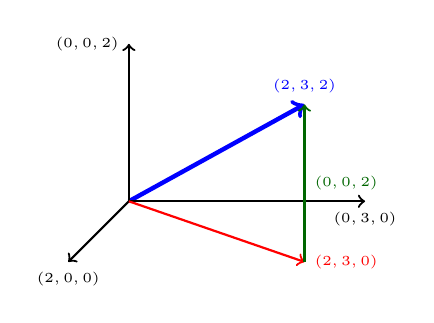
\begin{tikzpicture}[font=\tiny]

\onslide<2->{\draw[ultra thick,->][blue] (0,0,0) -- (3,2,2) node[above]{$(2,3,2)$};

\onslide<3->{\draw[ thick,->] (0,0,0) -- (3,0,0) node[below] at (3,0,0) {$(0,3,0)  $};
\draw[ thick,->] (0,0,0) -- (0,2,0) node[left] at (0,2,0){$(0,0,2)$};
\draw[thick,->] (0,0,0) -- (0,0,2) node[below]{$(2,0,0) $};}}

\onslide<4->{\draw[thick, ->] [red] (0,0,0) --(3,0,2) node[right] at (3,0,2){$(2,3,0)$};}
\onslide<5->{\draw[thick,->][dgreen] (3,0,2) -- (3,2,2) node[right] at (3,1,2) {$(0,0,2)$};}

\end{tikzpicture}
\end{column}
%\end{center} \pause
 \end{columns} 
 
\onslide<11->{Generalize by induction:} 
\onslide<12->{ Let $v=(x_1, \cdots, x_n)^T \in \BR^n$.} 
\onslide<13-> {Define 

$\| v\|  =} 
\onslide<14->{ \sqrt{\|\textcolor{red}{(x_1, \cdots, x_{n-1},0)}\|^2 + \|\textcolor{dgreen}{(0, 0,\cdots,x_n)}\|^2 }$} 

\onslide<15->{\hspace{1.5in}$ = \sqrt{\textcolor{red}{x_1^2 + \cdots +x_{n-1}^2}  + \textcolor{dgreen}{x_n^2}}$} 
\onslide<16->{$= \sqrt   {v^Tv}.$}
     
\onslide<17->{ The length (or norm) of a vector in $\BR^n$ is compatible with the vector space structure.} 
\onslide<18->{Let $v, w \in \BR^n$ and $c \in \BR$ then,}

\begin{itemize}
\onslide<19->{\item $\| v\|\geq 0 $} \onslide<20->{and $\|v\|=0 $ if and only if $v=0$}
\onslide<21->{\item $\|cv\| = |c| \|v\| $}
\onslide<22->{\item $\| v+w \| \leq \|v\| + \|w\|$} \onslide<23->{~~ (Triangle Inequality)}
\end{itemize}



\end{frame} %%%%%%%%%%%%%%%%%%%%%%%%%%%%%%%%%%%%%%%%



\begin{frame}
\frametitle{Orthogonal vectors in $\BR^n$}

\begin{columns}
\begin{column}{.48\textwidth}
\begin{center}
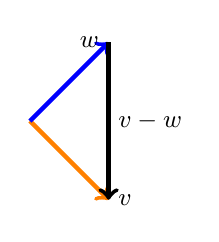
\begin{tikzpicture}[font=\small][baseline=(current bounding box.north), level/.style={sibling distance=50mm}]

\onslide<2->{
\draw[->] [orange] [ultra thick] (0,0) -- (1,-1) ;
\node [right] at (1,-1) {$v$};} 

\onslide<3->{
\draw[->] [blue] [ultra thick] (0,0) -- (1,1) ;
\node [left] at (1,1) {$w$};}

\onslide<7->{
\draw[->] [ultra thick] (1,1) -- (1,-1) ;
\node [right] at (1,0) {$v - w$};}

\end{tikzpicture}
\end{center}
\end{column}

\begin{column}{.58\textwidth}

\onslide<1->{We say vectors $v$ and $w$ in $\BR^n$ are orthogonal (perpendicular)} \onslide<4-> {$\Leftrightarrow$} 
\onslide<4->{ they satisfy the Pythagoras  theorem }\only<5->{$\Leftrightarrow$} 
\onslide<6->{$||v||^2  + ||w||^2 = }
\onslide<8->{ ||v - w||^2$  } 
\end{column}


\end{columns}
\onslide<8->{ \begin{eqnarray*}  
\Leftrightarrow \only<9->{ \|v\|^2 + \|w\|^2 & = &} \only<10->{ (v-w)^T (v-w) }\\  
\only<11->{& = &  (v^T-w^T) (v-w)} \\ \only<12->{ & = & v^T v-w^T
v  }\only<13->{-v^T w  + w^T w }\\ \  
\only<14->{& = & \|v\|^2 -2\ v^T w + \|w\|^2}  
\only<15->{ \text{~~~ (since $w^T v = v^T w$ )}} 
\end{eqnarray*} }\pause
\only<16->{Therefore, $v$ and $w$ are said to be {\it orthogonal} \pause if and only if }\only<17->{ \smallskip
\centerline{$ v^T w = 0.$ }\smallskip}

  
\only<18->{ \textcolor{dgreen}{\bf Q:} What can be said about Span$\{v\}$ and Span$\{w\}$ \pause} \only<19->{ when $v$ and $w$ are orthogonal to each other in $\BR^3$? } \pause \smallskip 
\end{frame} 

\begin{frame}
\frametitle{Orthogonal and Orthonormal Sets}\pause 
\textcolor{dgreen}{\bf Defn.} A set of {\it non-zero} vectors \pause $\{v_1, \cdots, v_k \}\subset \BR^n$, \pause is said to be an \textbf{orthogonal set} \pause 
if \textbf{ $ v_i^T v_j =0$  \pause for all $i, j= 1, \cdots n, \pause ~ i \neq j$}. \pause \smallskip


\textcolor{dgreen}{\bf Examples:} $\{ (1,3,1), (-1, 0,1) \} \subset \BR^3$, \pause $\{(2,1,0,-1), (0,1,0,1), (-1,1,0,-1) \} \subseteq \BR^4$, \pause 
$\left\{(\frac{1}{\sqrt{2}}, 0 ,\frac{1}{\sqrt{2}}),(\frac{1}{\sqrt{2}}, 0 ,\frac{-1}{\sqrt{2}})\right\} \subseteq \BR^3 $, \pause 
$\{ e_1, \cdots, e_n \} \subseteq \BR^n $. \pause \smallskip
  
Of these, the last two examples \pause have all unit vectors \pause (vectors of length one).  \pause
  
\textcolor{dgreen}{\bf Defn.} An orthogonal set $\{v_1, \cdots, v_k\}\subseteq \BR^n$ \pause with all unit vectors, \pause i.e., $\|v_i\|=1$ for all $i$, \pause is called an \textbf{orthonormal set}.\pause

\textcolor{dgreen}{\bf Note:} If $\{v_1, \cdots, v_k\}$ is an orthogonal set, \pause then $\{u_1, \cdots, u_k\}$ is orthonormal, \pause for $u_i = v_i/||v_i||$.

\end{frame} %%%%%%%%%%%%%%%%%%%%



\begin{frame}{Orthogonality and Linear Independence}
\only<2->{\textcolor{dgreen}{Theorem:} An orthogonal set in $\BR^n$ is linearly independent.} \smallskip

\only<3-22>{{\it Proof.}  \only<4->{Let $\{v_1, \cdots, v_k \}$ be an orthogonal set in $\BR^n$, }
\only<5->{i.e. $v_i\neq 0$  and }\only<6->{ $v_i^Tv_j=0$ for $i\neq j$. }\only<7->{ Note that for $i = j$, $v_i^Tv_i = ||v_i||^2  \neq 0$. }

\only<8->{Assume for some $a_1, \cdots, a_k \in \BR$,  }
\begin{eqnarray*}
\only<9->{a_1 v_1 + a_2 v_2 + \cdots+ a_k v_k  &=& 0 \\
\Rightarrow} \only<10->{  (a_1 v_1 + a_2 v_2 + \cdots+ a_k v_k )^T  v_1 
&= &  0\ v_1  =0 \\ }
\only<11->{\Rightarrow } \only<12->{ (a_1 v_1^T +a_2 v_2^T+ \cdots+ a_k v_k^T)\  v_1 & = & 0\\ }
\only<13->{\Rightarrow} \only<14->{  a_1 v_1^T v_1 +a_2 v_2^T v_1 + \cdots+ a_k v_k^Tv_1 &=&0 \\ }
\only<15->{\Rightarrow}\only<16->{  a_1 ||v_1||^2 & = & 0 \\ }
\only<17->{\Rightarrow }
\only<18->{ a_1 &=& 0  \text{ since }v_1 \neq 0 } 
 \end{eqnarray*}
\only<19->{ Similarly, we can show that $a_2=\cdots =a_n=0$.} 

\only<20->{Hence the set $\{v_1, \cdots, v_k \}$ is linearly independent.}} 

\end{frame}

\begin{frame}{Matrices with Orthogonal Columns}

\only<21->{ \textcolor{dgreen}{\bf True/False:} Any matrix whose columns form an orthogonal set is invertible.}
\only<22->{ Why? } \medskip

\only<23->{ $A=\left(\begin{matrix}
  2\\2\\1 \end{matrix} \pause ~~~ \begin{matrix} 1\\-2\\2 \end{matrix}
\pause ~~~ \begin{matrix} -2\\1\\2 \end{matrix}\right)$. } \smallskip
\only<24->{and $B=\left(\begin{matrix}
1\\1\\-1\\-1 \end{matrix}~~~ \pause \begin{matrix}
-1\\1\\-1\\1 \end{matrix} ~~~ \pause \begin{matrix} -1\\1\\1\\-1 \end{matrix}
 ~~~ \pause \begin{matrix} 1 \\ 1\\ 1\\ 1 \end{matrix}\right)$ } 
\only<25->{are both examples  of such matrices!}\smallskip

\only<26->{Let $A = [v_1~ \cdots~ v_n]$ be $m \times n$.} 
\only<27->{ If $\{v_1, \ldots, v_n\}$ form an {\it orthonormal} set in $\BR^m$, } 
\only<28->{ then $A^T A= \pause \begin{pmatrix}
  v_1^T \\ \vdots \\ v_n^T \end{pmatrix} \pause \begin{pmatrix} v_1 &
  \ldots & v_n \end{pmatrix} $}
  \only<29->{$ =
\begin{pmatrix} v_1^T v_1 & \ldots & v_1^Tv_n \\  \vdots & & \vdots \\
 v_n^T v_1 & \ldots & v_n^T v_n \end{pmatrix}$ } 
 \only<30->{$ = I_n$. }

\end{frame} %%%%%%%%%%%%%%%%%%%%%%%%%%%%%%%%5


\begin{frame}
\frametitle{Orthogonal Matrices}\pause

\textcolor{dgreen}{\bf Defn.} A square matrix $A$ whose column vectors form an
orthonormal set is called an {\bf orthogonal} matrix. \pause\medskip

If $Q = [u_1~ \cdots~ u_n]$ is an orthogonal matrix, then \pause 

$\bullet$  $\{u_1, \ldots, u_n\}$ is an orthonormal set \pause (by definition) \pause

$\bullet$  $Q^T Q = I = QQ^T$ \pause Why? \pause

$\bullet$ $\|Qx\|= \sqrt {(Qx)^T(Qx)} \pause = \sqrt {x^TQ^TQx} \pause=\sqrt {
x^Tx} = \|x\| $. \pause

$\bullet$  Row vectors of $Q$ are orthonormal \pause (since $QQ^T=I$). \pause  \smallskip

\textcolor{dgreen}{\bf Examples:}
1. $\left[\begin{array}{cc} \cos \theta & -\sin \theta \\ \sin \theta & \cos \theta \end{array} \right]$.\pause ~~~~~~ 
2.  $\dfrac 1{\sqrt 2}~ \begin{pmatrix} 1 & 1 \\ 1 & -1 \end{pmatrix}$.\pause\medskip


~~~~~~3. $\dfrac 1{3}~\left(\begin{matrix}
  2\\2\\1 \end{matrix} \pause ~~~ \begin{matrix} 1\\-2\\2 \end{matrix}
\pause ~~~ \begin{matrix} -2\\1\\2 \end{matrix}\right)$. \pause ~~~~~4.  $\dfrac 12 ~ \left(\begin{matrix}
1\\1\\-1\\-1 \end{matrix}~~~ \pause \begin{matrix}
-1\\1\\-1\\1 \end{matrix} ~~~ \pause \begin{matrix} -1\\1\\1\\-1 \end{matrix}
 ~~~ \pause \begin{matrix} 1 \\ 1\\ 1\\ 1 \end{matrix}\right)$.
\end{frame}

\end{document}


\end{document}
